\chapter*{Ejercicio 14}
\section*{Seno Función Armónica}

14. la figura 3 muestra un \textbf{modelo para la variación diurna} (i.e. durante un periodo de 24 horas) de la altura y de la marca sobre el  nivel medio del mar en una caleta de la bahía de San Francisco. Calcular los valores de $y_{0}$, la altura media; de la amplitud $A$, la frecuencia angular $\omega$ y la fase $\phi$ de una función armónica para el modelo con regla de correspondencia: \\
\[
y(t) = y_{0} + Asen(\omega t + \phi)
\]

\begin{center}
     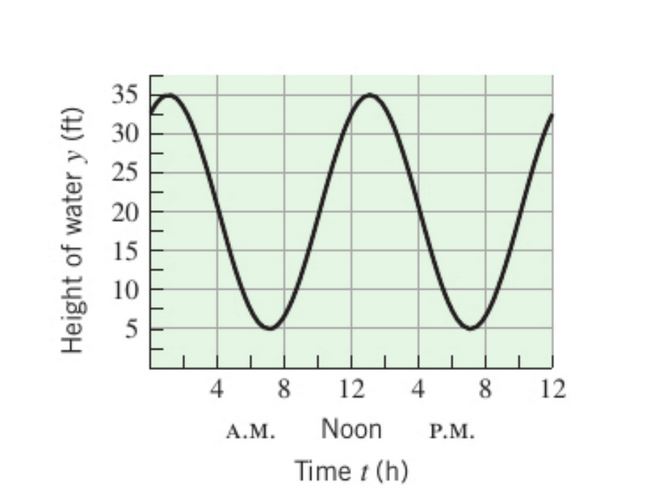
\includegraphics[width=10cm]{recursos/Grafica_seno.png}\par
\end{center}
si se supone que $t = 0$ corresponde a la media noche, el tiempo se mide en horas y la altura en pies.

\begin{center}
    \textbf{Calculo de las Transformaciones que sufre $sen(t)$ según la gráfica:}
\end{center}

Para la amplitud:
 \[
 A = \frac{max -min}{2}
 \]
\[
 A = \frac{35-5}{2}
 \]
 \[
 A = \frac{30}{2}
 \]
 \[
 A = 15
 \]
 Para $y_{0}$: \\
 Vmos que la altura media $y_{0}$ de la función esta situada en 20, Por lo tanto:\\
 \[
 y_{0} = 20
 \]

 Para la frecuencia angular $\omega$: \\
 Sambemos que el periodo $T$ de la función es igual a $12 horas$
 \[
 T = 12 hrs
 \]
 \[
 T = \frac{2\pi}{\omega}
 \]
 \[
 T = \frac{2\pi}{\omega}
 \]
 \[
 12 = \frac{2\pi}{\omega}
 \]
 \[
 \omega = \frac{2\pi}{12}
 \]
 \[
 \omega = \frac{\pi}{6}
 \]

Para la fase $\phi$: \\
En la gráfica podemos ver un desplazamiento hacia la derecha de 10 hrs con respecto a la gráfica de $sen(t)$ \\
Con esto decimos: \\
\[
\frac{\pi}{6} (t -10 )
\]
\[
\frac{\pi}{6}(t) - \phi
\]
\[
\frac{\pi}{6}(t - \frac{6\phi}{\pi})
\]
\[
10 = \frac{6\phi}{\pi}
\]
\[
10\pi = 6\phi
\]
\[
\phi = \frac{10\pi}{6}
\]
\[
\phi = \frac{5\pi}{3}
\]

Con todo esto podemos generar la función:
\[
y(t) = y_{0} + Asen(\omega t + \phi)
\]
\[
y(t) = 20 + 15sen(\frac{\pi}{6} t - \frac{5\pi}{3})
\]

\begin{center}
    \textbf{Transformaciones que sufre la función:}
\end{center}

\begin{center}
     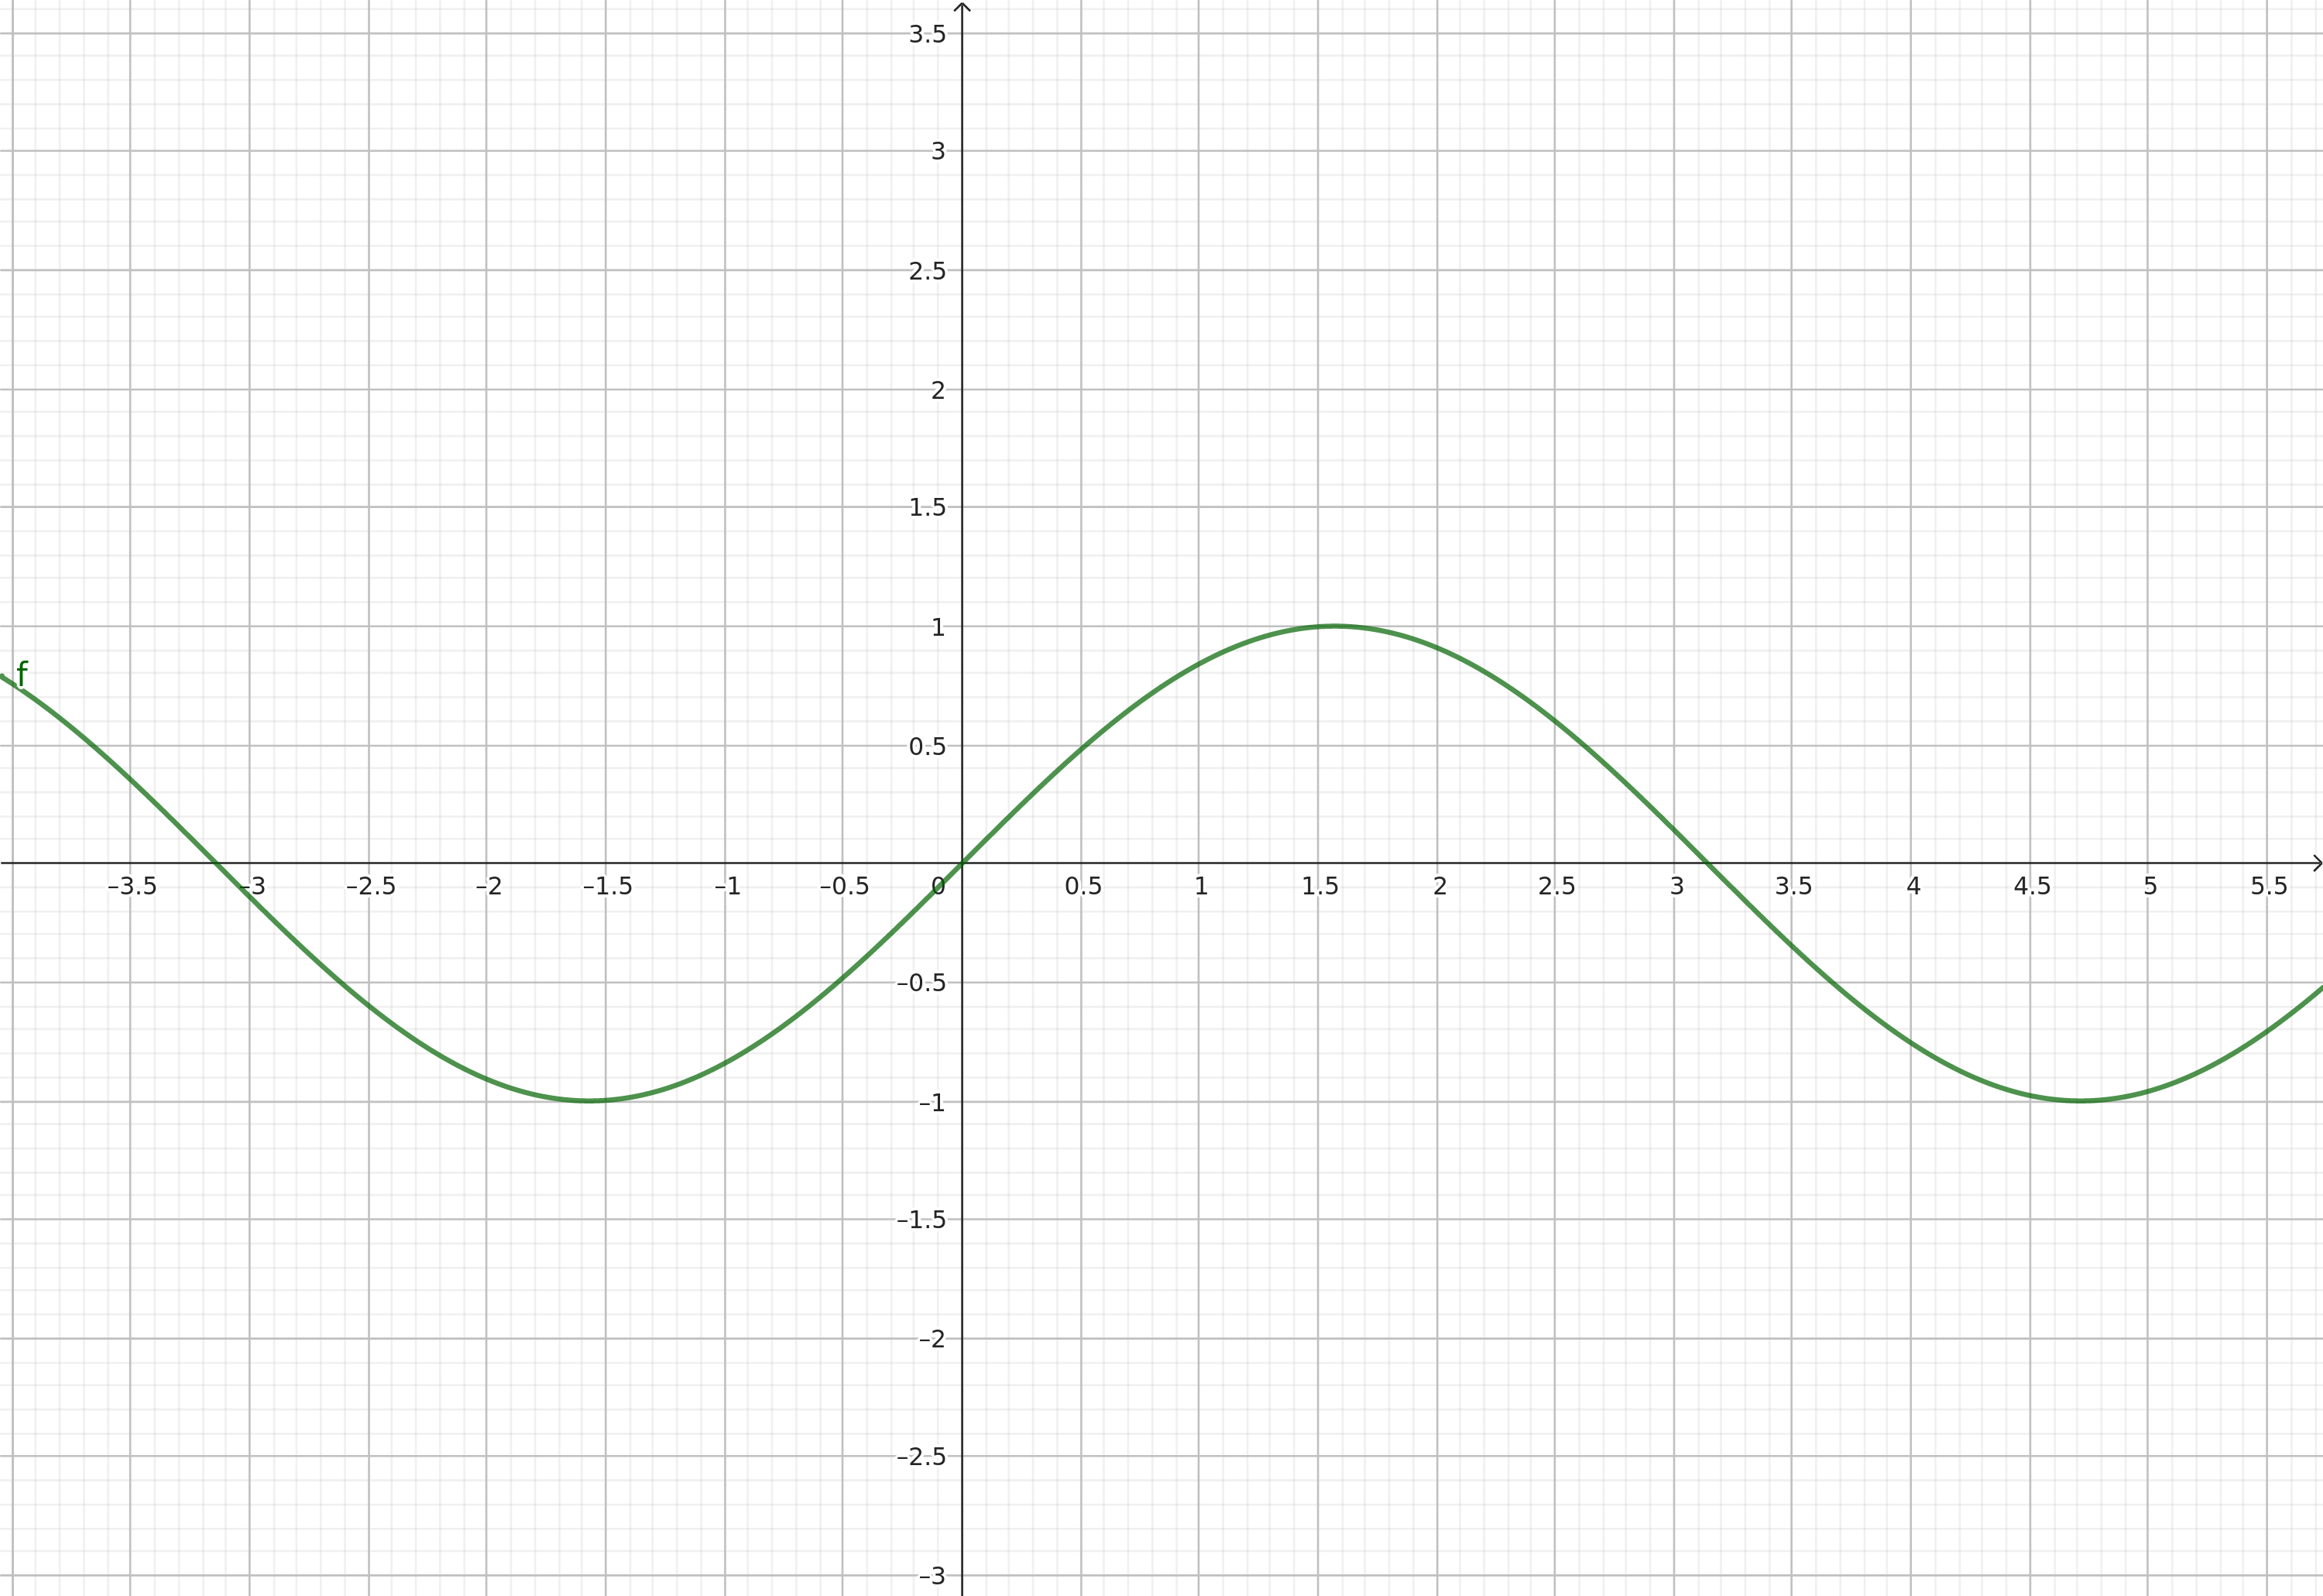
\includegraphics[width=10cm]{recursos/seno.png}\par
     $ y = sen(t) $
\end{center}

\begin{center}
     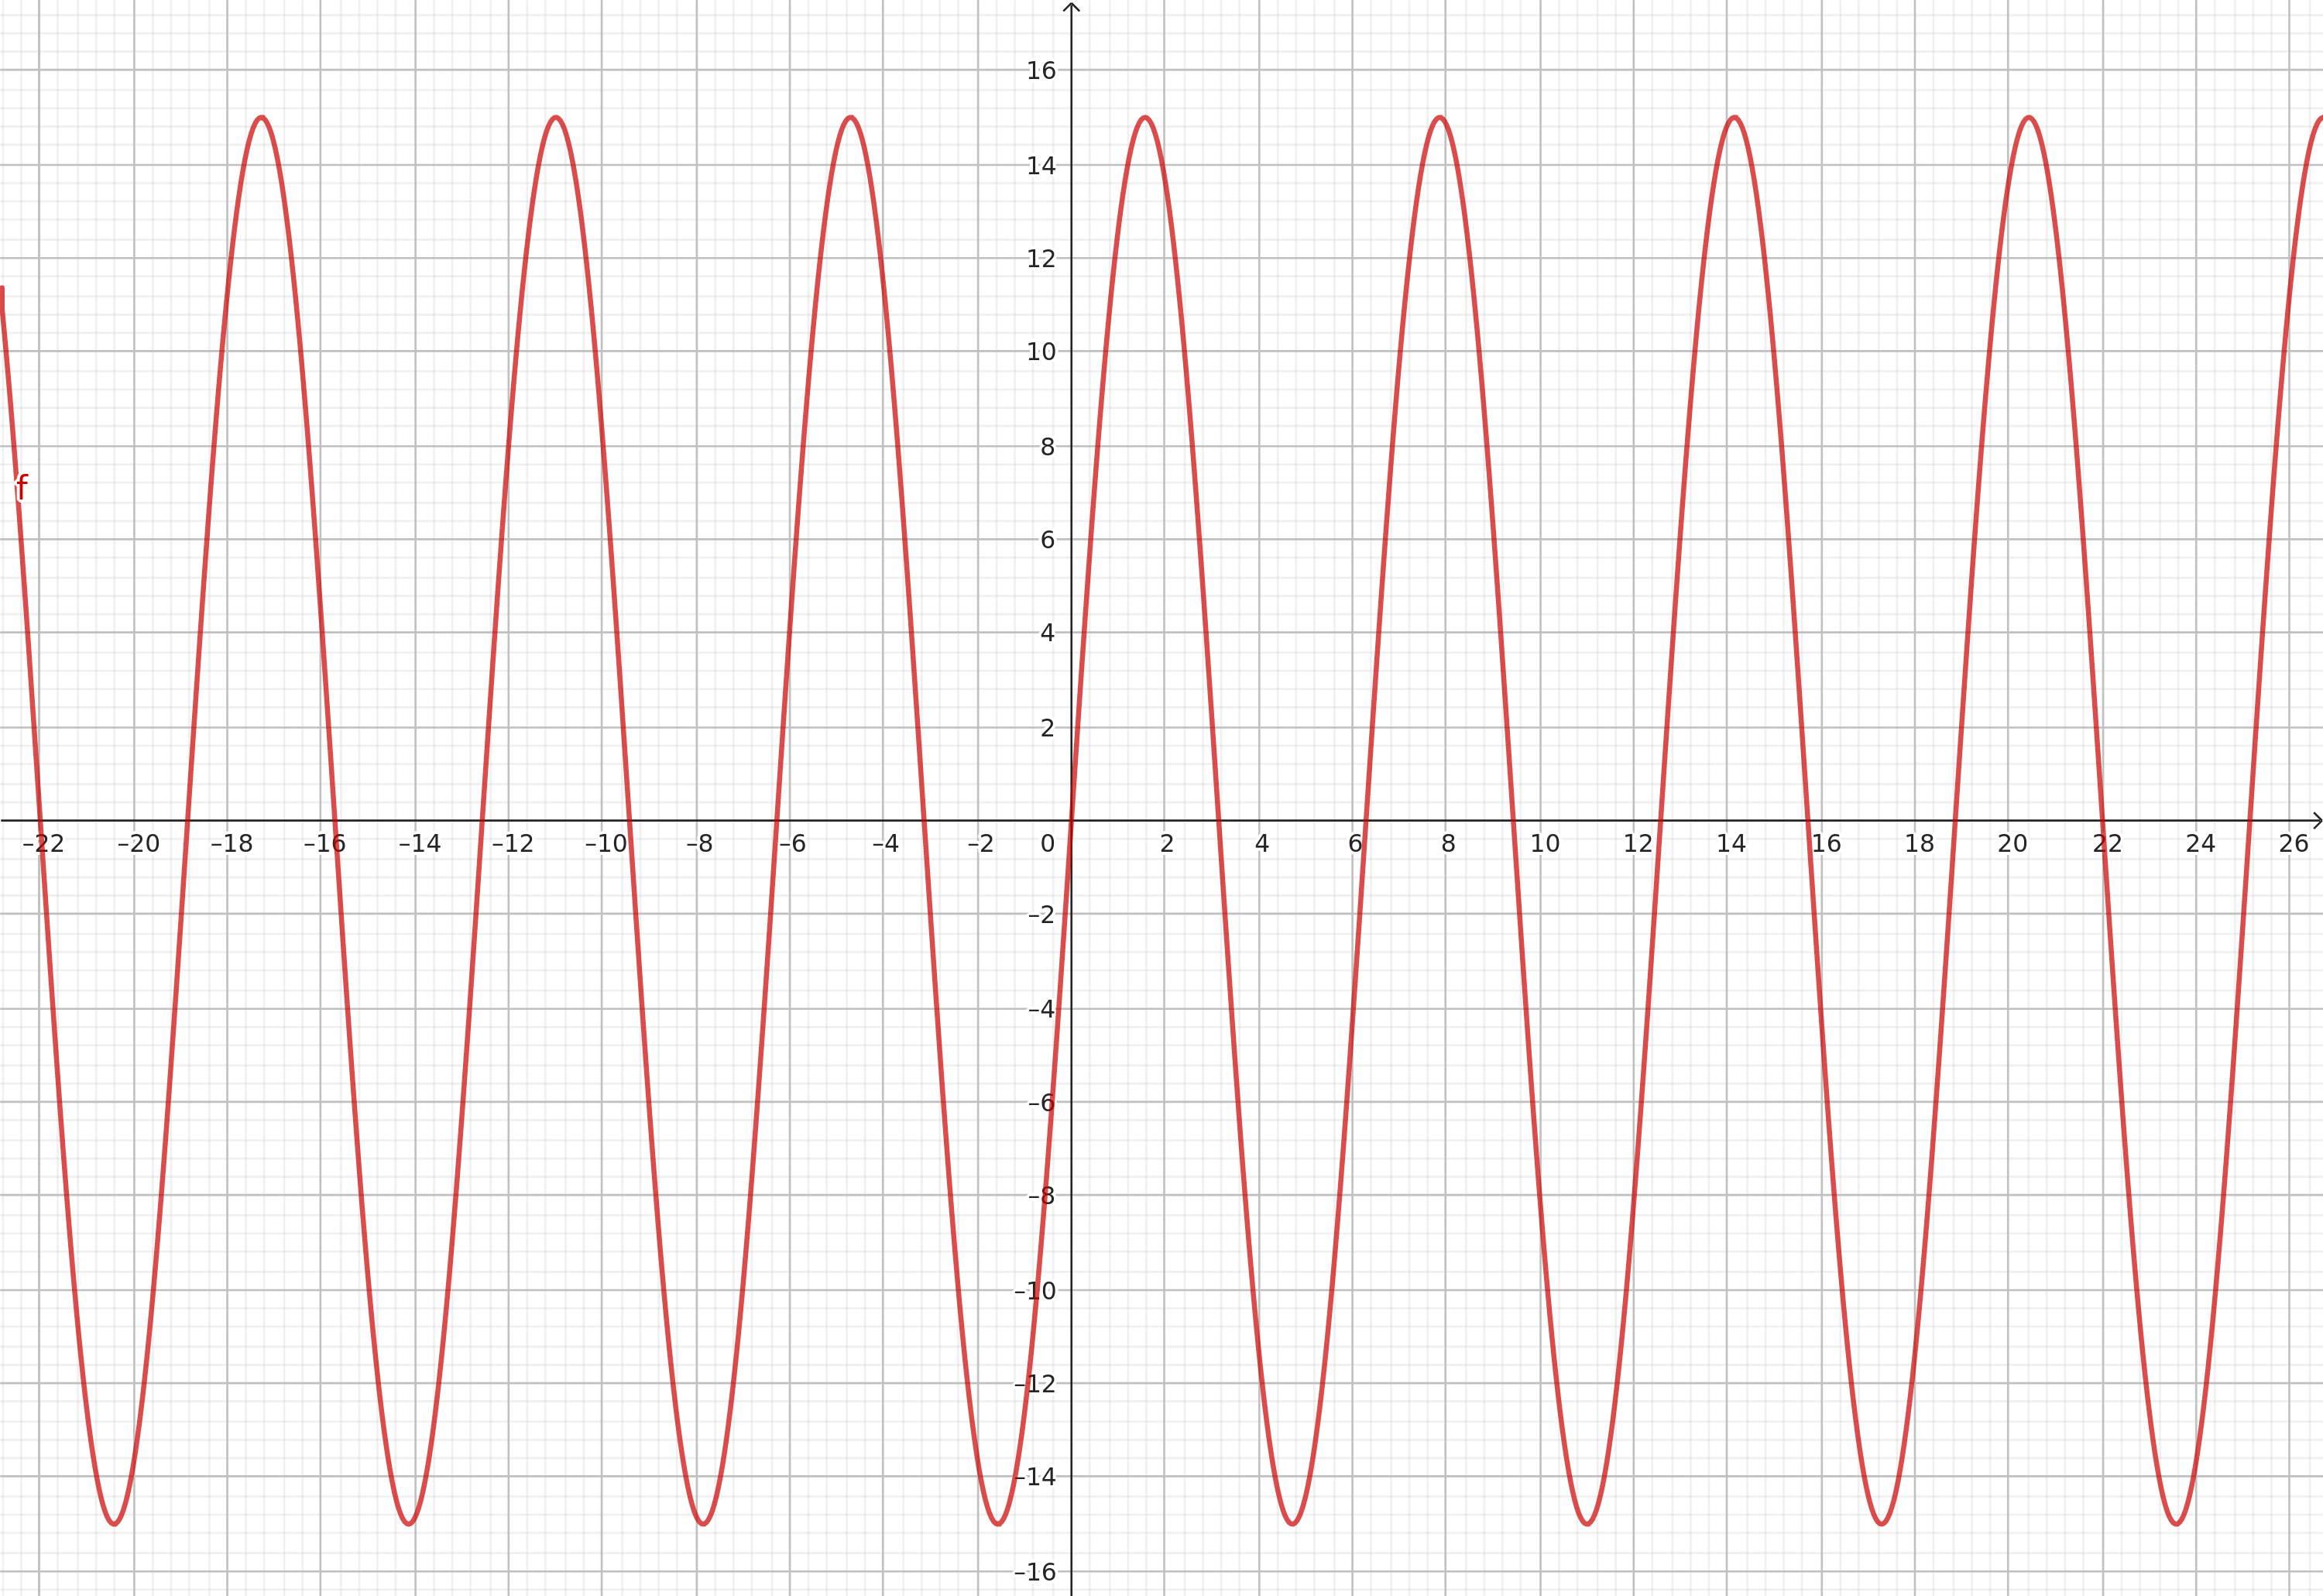
\includegraphics[width=10cm]{recursos/Aseno.png}\par
     $ y = 15sen(t) $
\end{center}

\begin{center}
     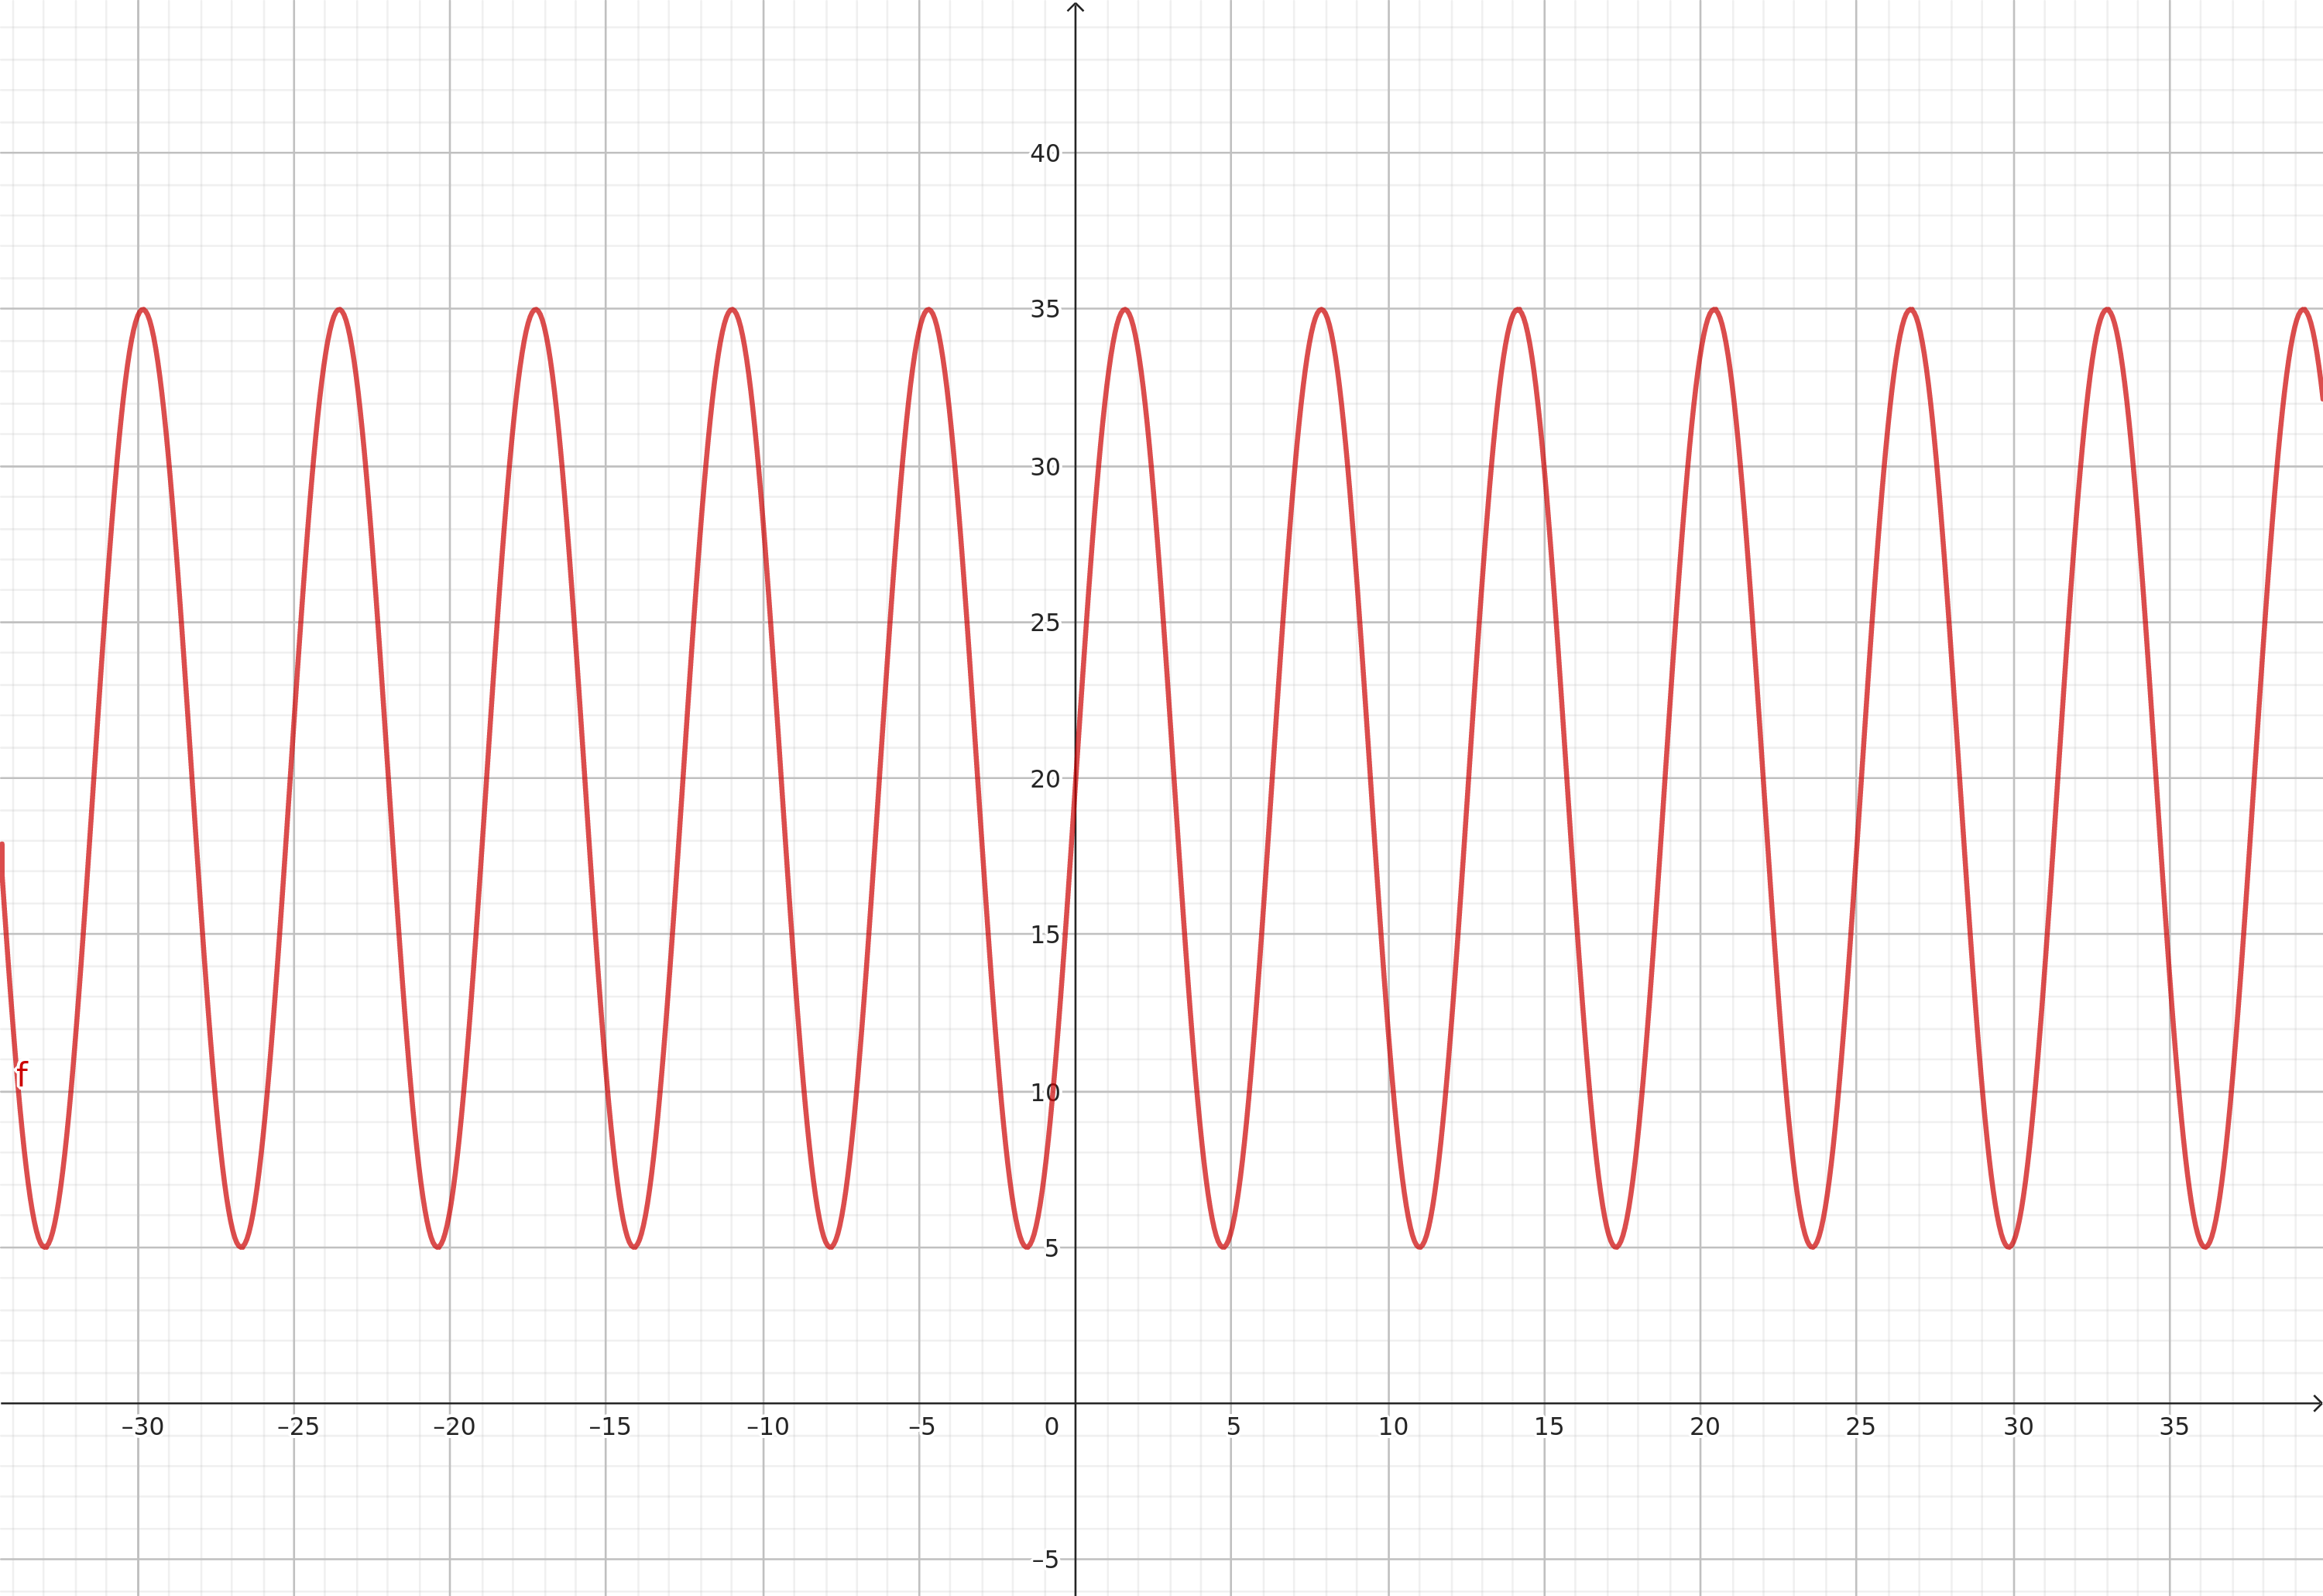
\includegraphics[width=10cm]{recursos/y_Aseno.png}\par
     $ y = 20 + 15sen(t) $
\end{center}

\begin{center}
     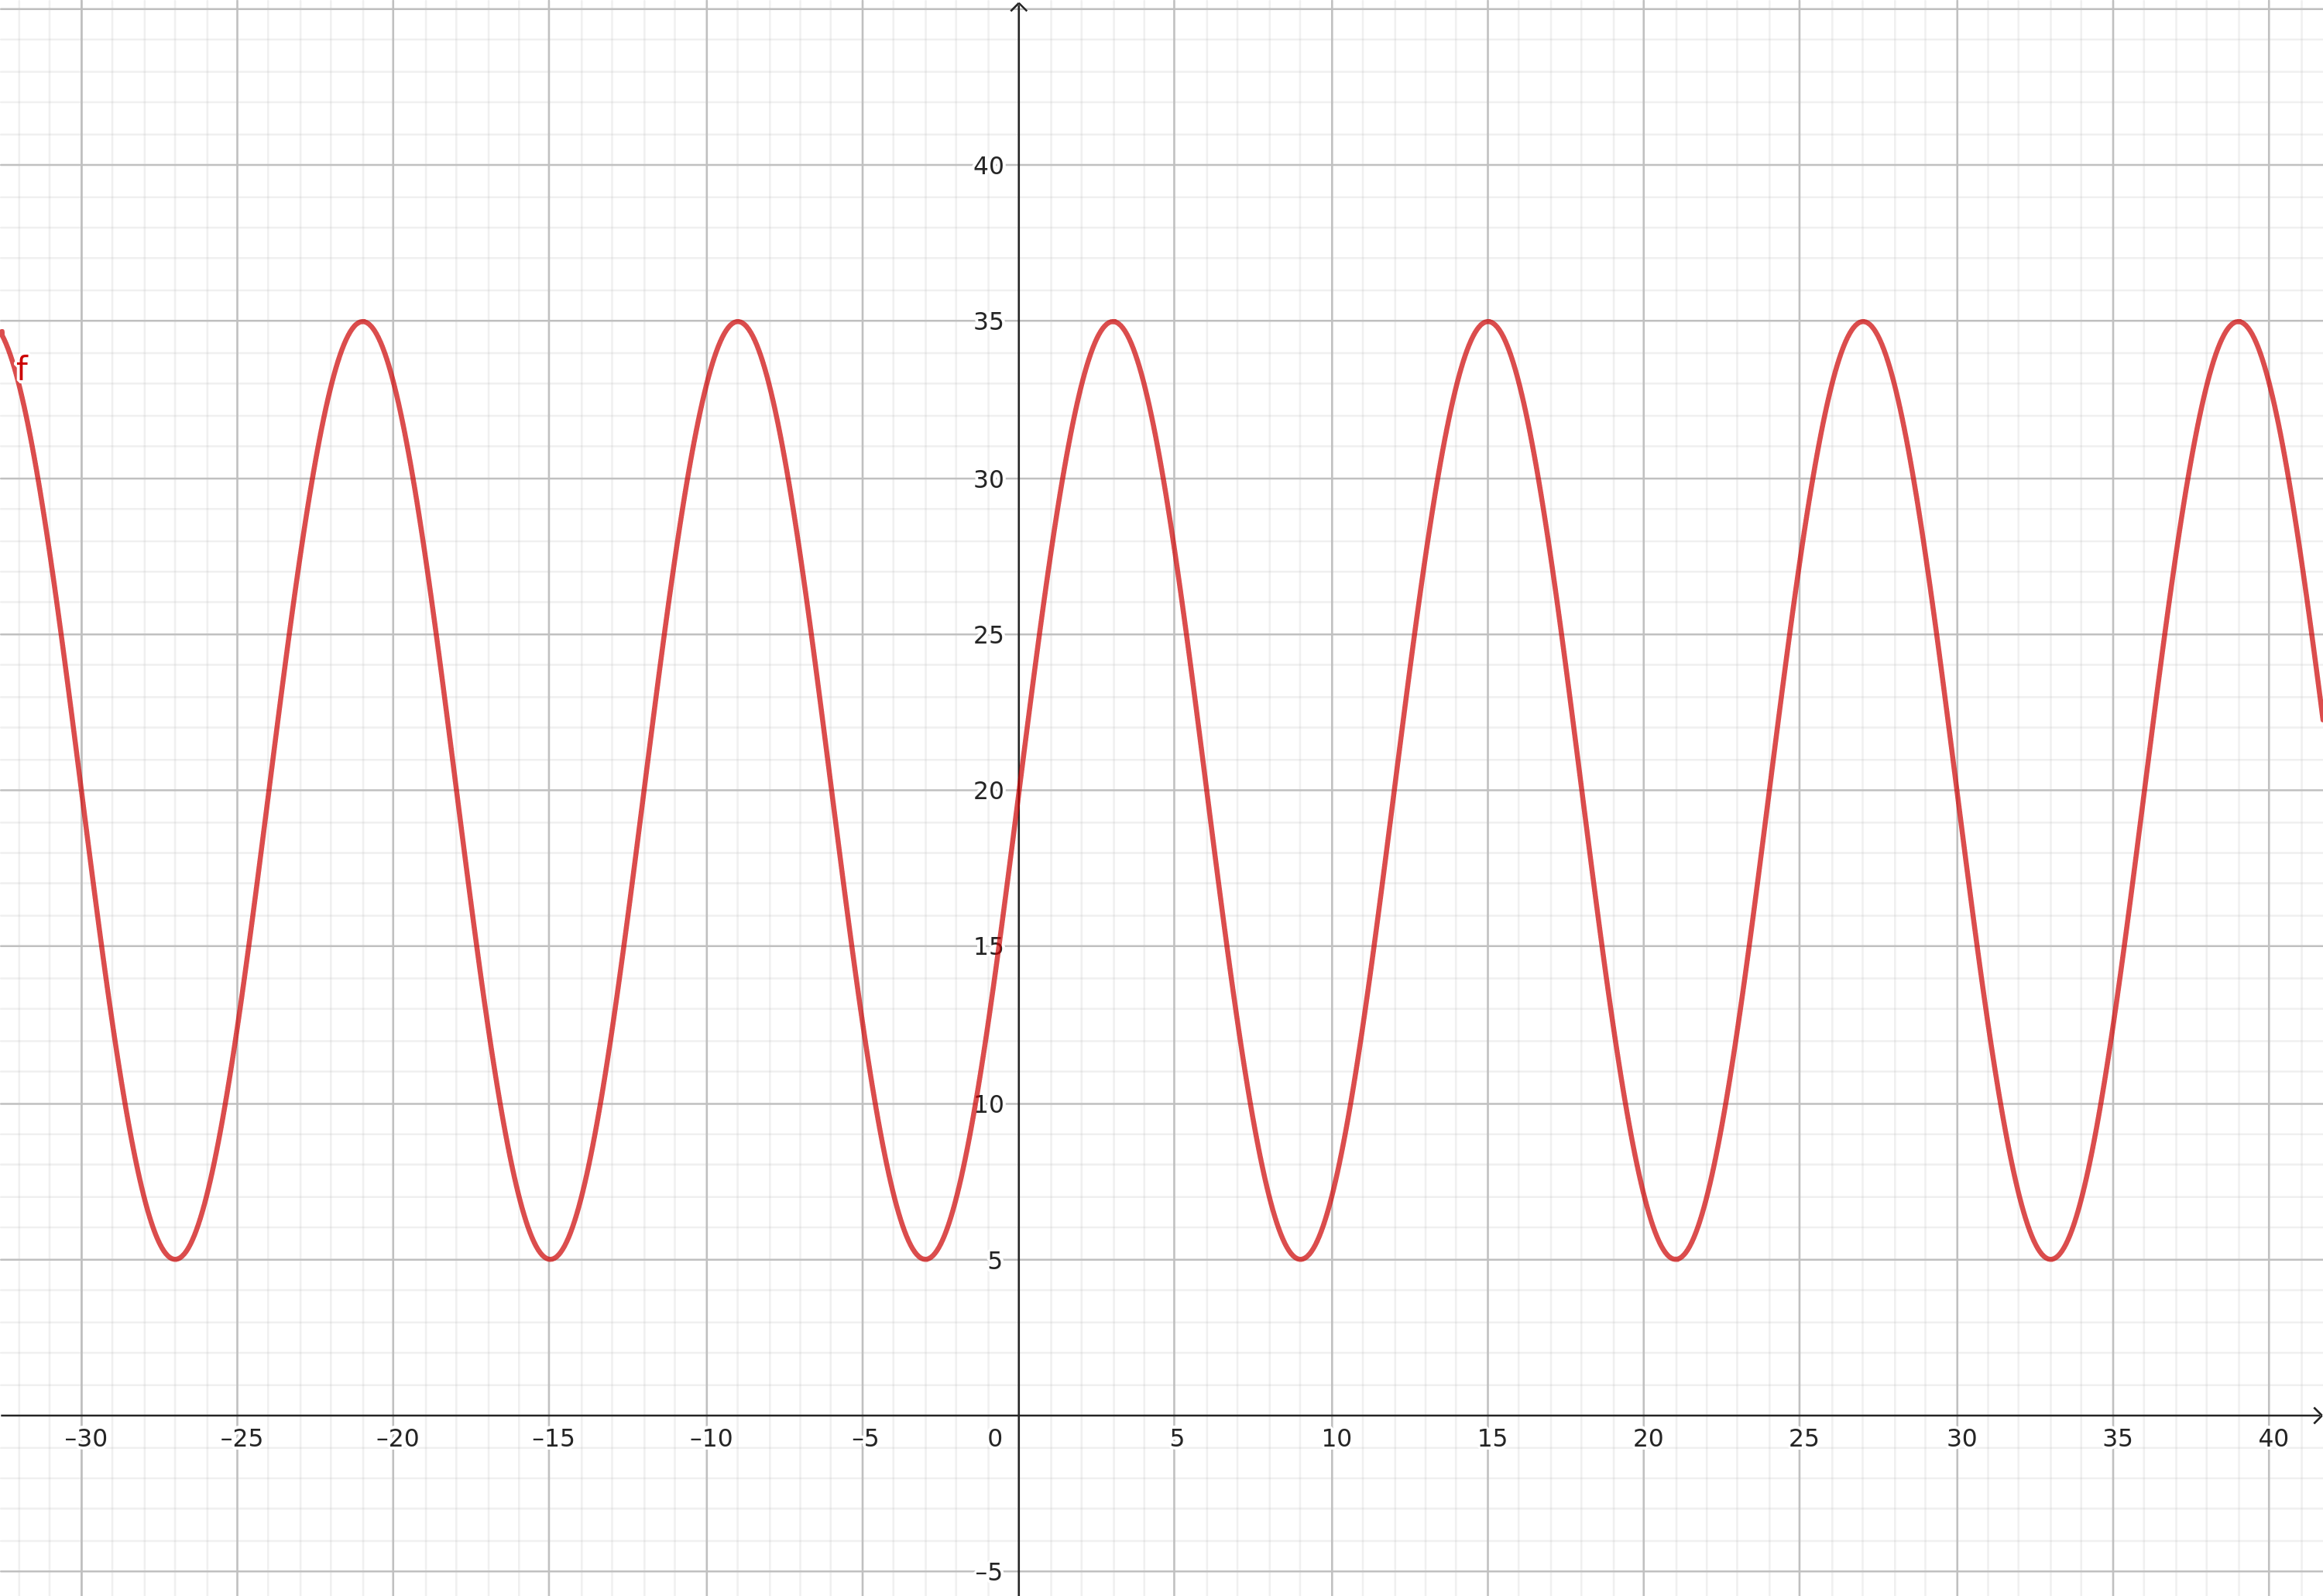
\includegraphics[width=10cm]{recursos/y_Aseno_o.png}\par
     $ y = 20 + 15sen(\frac{\pi}{6}t) $
\end{center}

\begin{center}
     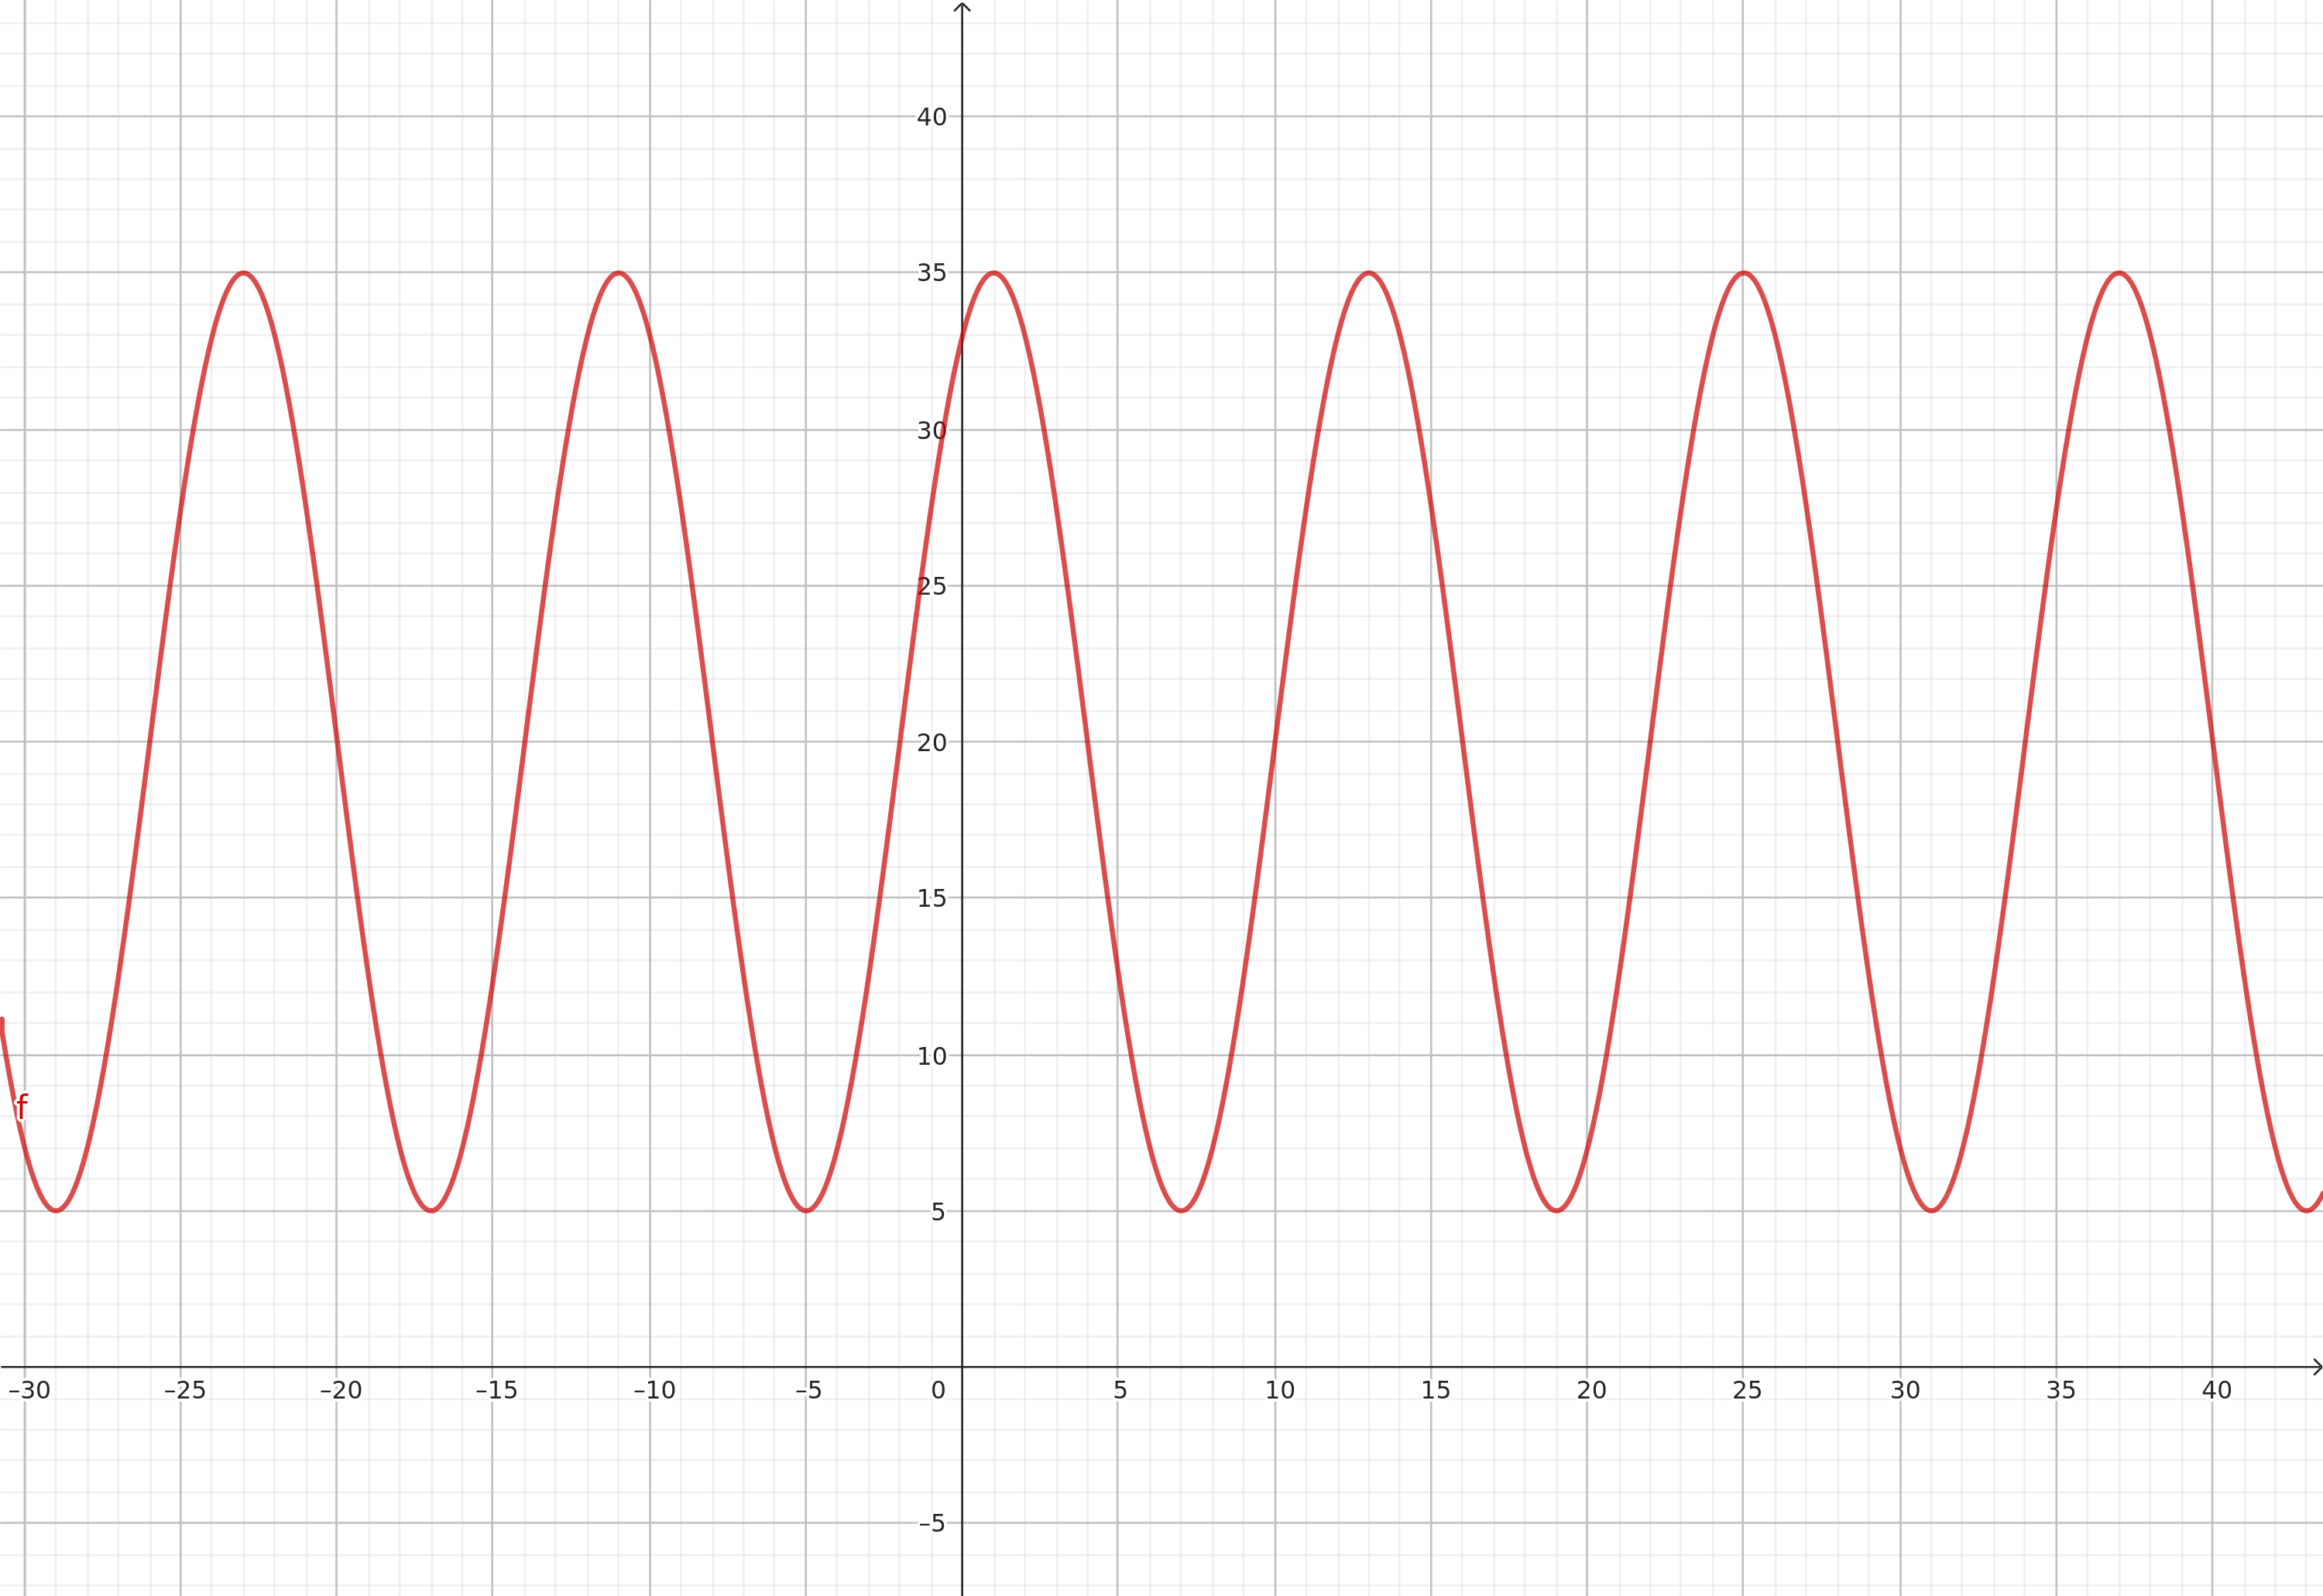
\includegraphics[width=10cm]{recursos/y_Aseno_o_phi.png}\par
     $ y = 20 + 15sen(\frac{\pi}{6}t - \frac{5\pi}{3}) $
\end{center}
\newline
\begin{center}
 Y obtenemos la gráfica del ejemplo.
\end{center}